\documentclass[runningheads]{llncs}
\usepackage{tikz}
\usetikzlibrary{bayesnet}
\usepackage{amsmath}
\usepackage{amsfonts}
\usepackage{rotating}
\usepackage{graphicx}
\usepackage{subfigure}
\usepackage{tikz}
\usepackage{multirow}
%\usepackage[linesnumbered,boxed]{algorithm2e}
\usepackage[ruled]{algorithm2e}
\usepackage{cite}
\setlength{\abovecaptionskip}{10pt}
\setlength{\belowcaptionskip}{-10pt}
\newcommand{\Ep}{\mathbb{E}}
\newcommand{\Real}{\mathcal{R}}
\newcommand{\Gaussian}{\mathcal{N}}
\usepackage{graphicx}
\usepackage{algorithmic}


\begin{document}
%title change
\title{Model Sentiment Evolution For Social Incidents}

%submission number
\author{Submission }
%anonymous
%\author{Yunjie Wang\inst{1} \and Xiaoli Wang\inst{1}\and Lin Sun\inst{2} \and Chen Lin\inst{1}}
%\authorrunning{Y.Wang et al.}
%\institute{Department of Computer Science, Xiamen University, China \email{chenlin@xmu.edu.cn} \and NatureWake Network Technology Co.,Ltd}

\maketitle             

\begin{abstract}
Modeling sentiment evolution for social incidents in microblogs is of vital importance for both researchers and government officials. 
Existing work on sentiment tracking is not satisfying, due to the lack of entity-level sentiment extraction and accurate sentiment shift detection.  
Identifying entity-level sentiment is challenging as microbloggers often use multiple opinion expressions in a sentence which targets towards different entities.
To address this problem, in this paper, we investigate the impact of proximity information to obtain more precise entity-level sentiment extraction.
Furthermore,detecting sentiment shift is not a trivial problem because the evolution of the background sentiment can not be ignored. 
We propose to simultaneously model the evolution of sentiment and sentiment shift by a state space model on the time series of sentiment polarities.
Experiments on a real data set demonstrates that the proposed methods outperform state-of-the-art methods.
\keywords{Sentiment Tracking  \and Dynamic Sentiment Model \and Opinion Analysis \and Microblog Mining }
\end{abstract}

\section{Introduction}
%Motivation
Nowadays Microblogging has become the major platform for Chinese people to publish information and share opinions about social incidents. Public opinion on Microblogging platforms has greatly influenced the Chinese society, for some incidents even change the investigation and judicial outcome~\cite{{Cheung2014Battle}}. 
For example, in 2010, Twenty-nine-year-old Li Changkui was originally condemned to immediate execution by a local court in Zhaotong because he killed a three-year-old boy and his teenager sister after raping her. The higher people's court of Yunnan later overruled the sentence and gave Li a two-year reprieve because he confessed his crime and gave compensation to the victims' family. 
The overruling caused great anger on microblogs with many arguing Li deserved to die for his brutality. 
Finally, the higher people's court of Yunnan overruled its previous decision and sentenced Li to death. 
The power of public opinion in Microblogging space makes it appealing to analyze sentiment evolution for social incidents in microblogs for individuals, enterprises, NGO organizations, researchers, government officials and so on.

%Problem studied
In this paper, to facilitate understanding of public opinions, we focus on the problem of modeling sentiment evolution for social incidents. 
Given a sequence of microblogging comments related to any social incident, our goal is to reveal the sentiment evolution pattern related to the involved entities in this incident and identify the significant sentiment shifts. 
As shown in Fig.~\ref{fig:tweet}, analysis of online comments on the murder case of Jiang Ge\footnote{The murder case of Jiang Ge, a Chinese student killed in Japan in 2016 has attracted wide attention online. Jiang was stabbed to death in her apartment by her roommate's boyfriend. After the tragedy, Jiang's mother (Jiang) blamed her daughter's roommate (Liu) for her daughter's death by claiming Liu had locked Jiang out when she was attacked.} leads to visualization of the evolution pattern of public sentiment towards the victim's mother (Jiang) and the victim's roommate (Liu). A sentiment shift is also detected in the third time point. %more specific, better describe the incident first

%background 
%opinion shift location
%Mrs. Jiang
%Jiang, Liu 
%related to Jiang
\begin{figure}
    \centering
    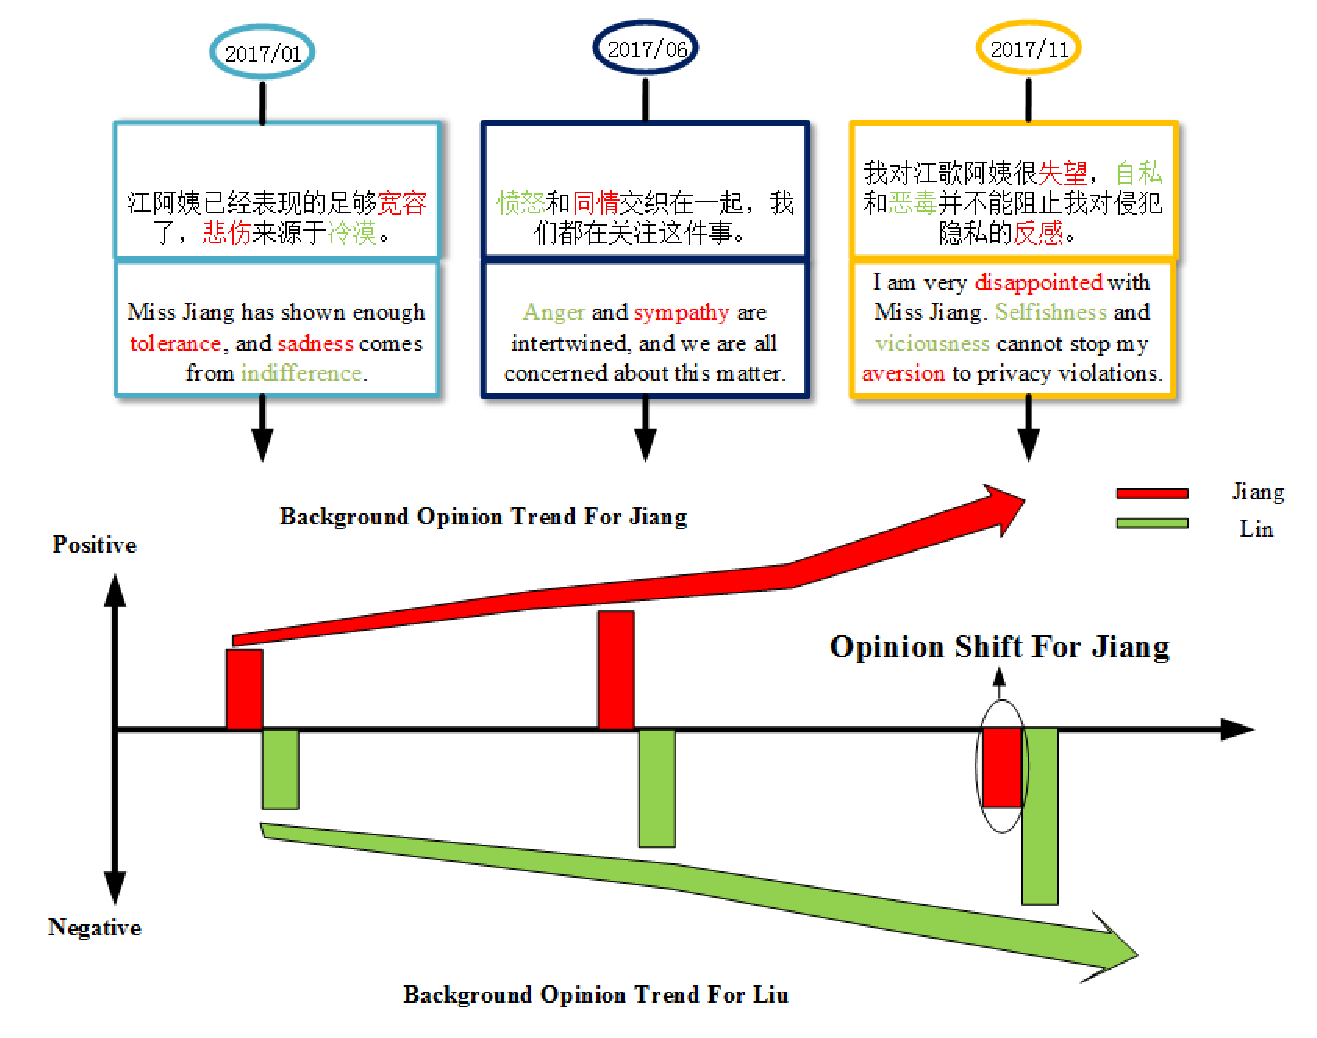
\includegraphics[width=1.0\textwidth,height=3.5in]{tweet.eps}
    \setlength{\abovecaptionskip}{-0.1cm}
    \caption{Comments from ``Jiang Ge'' incident and reflected characteristics of social incident.}\label{fig:tweet}
\end{figure}

%Related work
Recently there is an increasing interest in tracking microblogging sentiments for entities~\cite{Giachanou2016sentichange,Giachanou2017sentichange} or topics~\cite{Tsytsarau2014Topics,Thelwall2011topic}. Most of them are based on a two stage framework, i.e. first adopt a sentiment extraction tool such as SentiStrength~\cite{sentistrength2010} to compute the sentiment score for an entity or topic, then conduct statistical analysis such as outlier detection to obtain sentiment spikes. However, modeling public opinion for social incidents poses two challenges that haven't been addressed by previous research.

%mixed feelings
The first challenge is to \textbf{identify entity-level sentiment}. 
As a social incident often involves several entities (i.e. people or organizations), it is clearly problematic to utilize coarse-grained analysis which obtains an averaged sentiment for an event without separating different entities. %second layer
However, extracting entity level sentiment is not a trivial problem because the length limit of microblogs encourages people to use short and informal expressions.
Multiple opinion expressions are put in a sentence which targets towards different entities.
For example, as shown in Fig.~\ref{fig:tweet}, sentiment words for Jiang (in red) and for Liu (in green) are mixed together without a clear partition and a correct grammar structure. 
To address this challenge, it is helpful to \textbf{embed proximity information} to enhance entity-level sentiment extraction accuracy. 



%background evolution + shift
The second challenge is to \textbf{detect sentiment shift}.
In previous work, researchers mostly depend on statistical analysis such as outlier detection to detect sentiment spikes~\cite{Giachanou2016sentichange,Giachanou2017sentichange,Giachanou2016sentitime}.
Such a method is not sufficient, because the evolution of the background is largely overlooked.
The fact that events are continuously changing causes changing responses in public opinions. Hence sentiment shift should be distinguished with the evolution patterns of background sentiment.  
For example, in Figure~\ref{fig:tweet}, the background sentiment towards Jiang is an increasing trend of positive sentiment. Revealing this evolution pattern marks the significance of sentiment shift at the third time point. %running example
In this article we propose a probabilistic model that \textbf{simultaneously model the evolution of background opinion and the opinion shifts}.

%contributions
Our contributions are two folds. 
\textbf{In the application aspect}, we explore the feasibility of tracking sentiment evolution for social incidents on Chinese microblogs. Our work sheds insights into better understanding public opinions and provides a solid foundation for future applications such as explaining the causes of sentiment shifts. 
\textbf{In the model aspect}, we propose to simultaneously model the evolution of background sentiment and sentiment shift by state space models on the natural parameters of the binomial distributions that represent the sentiment polarity. 
Furthermore, we investigate the impact of proximity information in obtaining entity-level sentiment extraction.


This paper is organized as follows. We briefly survey the related work in Sec.~\ref{sec:related}. In Sec.~\ref{sec:sentiment classification} to Sec.~\ref{sec:public opinion model}, we describe the methodology. We present and analyze the experimental results on a real data set in Sec.~\ref{sec:Experiment}. We conclude our work and suggest future directions in Sec.~\ref{sec:conclusion}.


\section{Related Work}\label{sec:related}
%sentiment tracking
\textbf{Sentiment Tracking on Microblogs} has received considerable attention from both academy and industry~\cite{Giachanou2016sentichange,Giachanou2017sentichange,Giachanou2016sentitime,An2014sentimentchange,Bollen2011sentimentchange,Tan2014topic,Montero2016sentimentchange}. Most of existing work adopt a cascade framework, i.e. in the first step sentiment of each tweet is extracted, in the second step sentiment shift is detected~\cite{Giachanou2016sentichange,Giachanou2017sentichange,Giachanou2016sentitime,An2014sentimentchange,Bollen2011sentimentchange,Tan2014topic}. To extract sentiment, the collection of tweets are divided into numerous time slices, and the ratio of positive and negative sentiments is computed in a time slice~\cite{Giachanou2017sentichange,Giachanou2016sentitime,An2014sentimentchange,Bollen2011sentimentchange}. 
To detect sentiment shift, residual between actuarial and predicted sentiment value is the most commonly adopted measurement~\cite{Giachanou2016sentichange,Giachanou2016sentitime}. 
Furthermore, topic information is incorporated in recent studies. Sentiment change is represented by topic changes in~\cite{Tan2014topic}, an integrate framework based on empirical heuristics is utilized in~\cite{Montero2016sentimentchange} to identify
the emotional spikes and locate causes of spikes.%integration 

%sentiment analysis
A fundamental block in sentiment tracking systems is \textbf{sentiment analysis}. In the literature, there are two types of sentiment analysis algorithms: supervised learning and lexicon-based methods~\cite{Ahmed2017SentiCR}. \textbf{Supervised learning method} creates a training model based on training data
to classify the sentiment polarity of sentences. Obtaining training data and selecting features are the two most important parts of this methods. 
Emoji is often used to label sentiments of tweets~\cite{Go2009Supervisedlearning,Pak2010Supervisedlearning}. Hashtag is another major source to label training data~\cite{Papadopoulos2012SocialEvent}.
But the accuracy of label by emoji is low. To overcome this issue, an ensemble of sentiment detection tools is employed to obtain the training data~\cite{Barbosa2010Supervisedlearning}. 
The goal of supervision based methods is to classify the polarity of sentiments. To obtain a high precision, lexical features such as unigrams and POS~\cite{Go2009Supervisedlearning,Davidov2010Supervisedlearning}, syntax features such as retweets, URLs, emoticons, and meta-features such as POS tags, words’ polarity,~\cite{Barbosa2010Supervisedlearning} are obtained.
Experiments have shown that classifiers benefit most from features which involve text polarity~\cite{Agarwal2010Supervisedlearning}.

Due to the lack of training data, most researchers turn to \textbf{lexicon based methods}. 
SentiStrength is the first open domain large-scale lexicon, which is used as a baseline in most sentiment detection algorithms like SentiStrength2~\cite{Thelwall2012lexicon}, SentiStrength-SE~\cite{Rakibul2017SentiStrength-SE}, and VADER~\cite{Hutto2014SSimproved}. 
SentiStrength2~\cite{Thelwall2012lexicon} improves the accuracy of SentiStrength by adding idioms. 
VADER~\cite{Hutto2014SSimproved} improves the accuracy of SentiStrength by grouping sentiment words on Twitter and manually filtering them. 
SentiStrength-SE improves the recall of SentiStrength by designing different lexicons for different domains~\cite{Rakibul2017SentiStrength-SE}. 
The above methods are based on static lexicons.
Recently,we've seen an emerging attempt to construct dynamic lexicon. 
For example, to enclose subtle dimensions of a word’s sentiment, a seed lexicon is defined in ~\cite{Feng2011lexicon} and connotation lexicon is retrieved based on PageRank and HITS. 
%However, such a connotation lexicon is still noisy and often not scalable, because it contains sentiment words that are not related to any entity in an event.
However, directly applying these lexicons does not guarantee the accuracy of entity level sentiment extraction, because opinion expressions towards different entities are usually mixed together in a microblogging post. 


\section{Proximity-based Entity-level Sentiment Extraction}\label{sec:sentiment classification}


\subsection{Problem Definition}
%$D$ source
In this section, we describe Proximity-based Entity-level Sentiment Extraction (PESE). Suppose we have a collection of incident relevant microblog posts $O=\{o\}$ . As an incident involves several entities $E=\{e\}$, we can represent each post $o$ as a set of sentiment triples and entity triples, $o=\{(w_i,l_i,v_i)\}\bigcup \{(e_j,l_j)\}$, where $i$ is the index for sentiment words, $w_i$ is the word which is extracted from a sentiment lexicon $w_i\in D$,  $l_i$  is the location and $v_i$ is the sentiment value of $w_i$, which is also extracted from a sentiment lexicon, $v_i \in \mathcal{R}$,  $j$ is the index for entity occurences, $e_j\in E$ is the name of the entity, $l_j$ is the location of the entity in the post. Our aim is to output the sentiment polarity $p$ for the entity $e_j$ in the post $p_e(o)\in\{0,1\}$.
\vspace{-0.6cm}
\subsection{Distance Function}

%assumption
Our basic assumption is that the position of a sentiment word influences the performance of entity-level sentiment extraction. Intuitively, the closer a sentiment word is to an entity, the more likely the sentiment word is to describe the entity. Inspired by~\cite{Lv2009distancefunction}, given two locations $l_i,l_j$, we use four distance kernel functions to compute influence of sentiment words on entities, namely Gaussian, Triangle, Cosine, and Circle:

%notations
\textbf{1. Gaussian kernel}
\begin{equation}
    k(l_i,l_j) = \exp\left[\frac{-(l_i-l_j)^2}{2\sigma^2}\right],
\end{equation}

\textbf{2. Triangle kernel}
\begin{equation}
k(l_i,l_j)=\begin{cases}
1-\frac{|l_i-l_j|}{\sigma} &\mbox{if $|l_i-l_j|\leq \sigma$}\\
0 &\mbox{otherwise},
\end{cases}
\end{equation}

\textbf{3. Cosine (Hamming) kernel}
\begin{equation}
k(l_i,l_j)=\begin{cases}
\frac{1}{2}\left[1+cos\left(\frac{|l_i-l_j|\cdot\pi}{\sigma}\right)\right] &\mbox{if $|l_i-l_j|\leq \sigma$}\\
0 &\mbox{otherwise},
\end{cases}
\end{equation}

\textbf{4. Circle kernel}
\begin{equation}
k(l_i,l_j)=\begin{cases}
\sqrt{1-\left(\frac{|l_i-l_j|^2}{\sigma}\right)} &\mbox{if $|l_i-l_j|\leq \sigma$}\\
0 &\mbox{otherwise},
\end{cases}
\end{equation}

Note that all four of these kernel functions are governed by one parameter $\sigma$, which is tuned in the experiment.
To obtain the proximity influence between an entity $e$ and a sentiment word $w$, we compute the average distance over its multiple occurrences, that is $d(e,w)=\sum_{l_i,l_j} k(l_i,l_j)/(n_i\times n_j)$, where $l_i$ is the location of each occurrence of sentiment word $w$, $l_j$ is the location of each occurrence of entity $e$, $n_i$ is the number of occurrences of $w$ and $n_j$ is the number of occurrences of $e$ %multiple occurrence

\subsection{Entity Level Sentiment Polarity Classification}

To classify the polarity $p_e(o)$ of sentiment towards an entity $e$ in a post $o$, we first obtain an entity-level sentiment value by calculating the average of the influence  on the entity from different sentiment words. $n_i$ is the number of anti-words and $d_i$ is the sum of value of degree words between $i$th sentiment word and $(i-1)$th sentiment word. N is the number of sentiment words.

%multiple entities


\begin{equation}\label{equ:entitysentiment}
s = \frac{\sum_{i=1}^{N}(-1)^{n_i}\cdot d_i\cdot v_i\cdot k(l_i,l_j)}{N}
\end{equation}

%
if the sentiment value $s>0$, the sentiment polarity of this sentence is positive $p_e(o)=1$. if the sentiment value $s<0$, the sentiment polarity of this sentence is negative $p_e(o)=0$. %output 


\section{Public Sentiment Evolution Model}\label{sec:public opinion model}
\subsection{Problem Definition}
In this section, we describe how to model public sentiment evolution. For a social incident which involves several entities $E=\{e\}$, we first divide the collection of tweets to $T$ time slices. %divide?
Suppose in each time slice, there are $N_t$ posts, where each post is pre-processed by the PESE to observe an entity-level sentiment polarity on each post $p\in \{0,1\}$. 
We build a public sentiment evolution model for each entity.
Our assumptions are: (1) there is a background opinion distribution, i.e. how users normally react to the entity. 
(2) The background is smoothly and slowly changing. 
(3) However sometimes a sudden shift on public opinions appears, i.e. triggered by sometimes a new piece of evidence.  

Therefore, we present the following generation process, as illustrated in Figure~\ref{fig:opinion}.

\begin{figure}[htp]
  \centering
  \tikz[scale=0.3]{ %
%hypers
    \node[const] (a) {$a$} ; %
        \node[const,right = of a] (b) {$b$} ; 
        \node[const,right = of b](sigma){$\sigma^2$};
        
%emotion evolutions        
  \node[latent, below = of b](gamma){$\gamma$};

   \node[latent, below = of sigma](alpha0){$\alpha_0$};
     \node[const, right = of alpha0](alphadots){$\cdots$};
   \node[latent, right = of alphadots](alphat){$\alpha_t$};
    \node[latent, right = of alphat](alphatp){$\alpha_{t+1}$};
    
    \edge{a}{gamma};
     \edge{b}{gamma};
     
      \edge{sigma}{alpha0};
    	\edge{sigma}{alphat};
	\edge{sigma}{alphatp};
	\edge{alpha0}{alphadots};
	\edge{alphat}{alphatp};
    
  	\node[latent, below = 1 of gamma] (s0) {$s_{0,n}$};
%	 \node[latent, below = 0.8 of alpha0] (eta0) {$\eta_0$};
       	\edge{gamma}{s0};
%    	\edge{alpha0}{0};        
	

%	 \node[latent, below = 0.8 of alphat] (etat) {$\eta_t$};
	 		\node[latent, right = 2.8 of s0 ] (st) {$s_{t,n}$};
        	\edge{gamma}{st};
%            	\edge{alphat}{etat};

	
        \node[latent, below = 2 of alpha0 ] (y0) {$p_{0,n,m}$};
            \node[latent, below = 2  of alphat ] (yt) {$p_{t,n,m}$};
       	\edge{s0}{y0};
	\edge{alpha0}{y0};
	    	\edge{st}{yt};
	\edge{alphat}{yt};
	
	 \plate[inner sep=0.1cm, xshift=-0cm, yshift=0 cm] {O0} {(y0)} {$M_n$};
		 \plate[inner sep=0.1cm, xshift=-0cm, yshift=0.12 cm] {S0} {(s0)  (O0) } {$N_0$}; 

		 \plate[inner sep=0.1cm, xshift=-0cm, yshift=0 cm] {Ot} {(yt) } {$M_n$};
		 \plate[inner sep=0.1cm, xshift=-0cm, yshift=0.12 cm] {St} {(st)  (Ot) } {$N_t$}; 
	
        \node[latent, below = 2 of y0 ] (beta) {$\beta$};
        
       	\edge{beta}{y0};
	\edge{beta}{yt};
	   \node[latent, below = of beta](c){$c$};
	      \node[latent, right = of c](d){$d$};
   	\edge{c}{beta};
	\edge{d}{beta};
       
     }
 \caption{Plate notation of the proposed opinion evolution model}\label{fig:opinion}
\end{figure}

\vspace{-0.6cm}
\begin{itemize}
\item For time $t=0$, sample  for the public opinion distribution, $\alpha_0\sim \Gaussian(0,\sigma^2 I)$.
\item For items $t=1: N$, sample $\alpha_{t+1}\sim \Gaussian(\alpha_t,\sigma^2)$. As $\Gaussian$ is a continuous and differentiable distribution, the evolution of background opinions is smooth and slow.
\item Generate a global prior for the switch, i.e. a variable that controls how likely the public opinion to change, by $\gamma\sim Beta(a,b)$
\end{itemize}
\begin{itemize}
%notations
\item For each pieces of evidence
\begin{itemize}
\item Generate a switch $s_t \sim Bern(\gamma)$
\item For each observation, generate $p_{t,n,m}\sim \begin{cases}
Bern(\pi(\alpha_t)) & \text{ if } s_{t,n}= 1\\ 
Bern(\beta) & \text{ if } s_{t,n}= 0 
\end{cases}$
\end{itemize}
\end{itemize}


%y -> p
% M_n -> plate removed



\vspace{-0.6cm}
\subsection{Inference}
The joint probability is given by
%notations
\begin{multline}
    p(\gamma,\beta,\alpha_0,\cdots,\alpha_T, \vec{s},\vec{p}, |a,b,c,d,\sigma^2) \\
    =    p(\gamma|a,b) p(\beta|c,d)  p(\alpha_{0:T}|\sigma^2) \prod_t \prod_ n p(s_{t,n}|\gamma) \prod_m p(p_{t,n,m}|s_{t,n},\alpha_t,\beta) 
\end{multline}
\vspace{-0.6cm}


    
In the nutshell, the optimization algorithm follows the framework of variational inference. Thus we make the following assumptions. 

\vspace{-0.6cm}
\begin{equation*}
q(Z|\vec{p},a,b,c,d,\sigma^2) = q(\gamma|\hat{a},\hat{b}) q(\beta|\hat{c},\hat{d}) q(\alpha_{0:T}|\hat{\alpha_{0:T}})\prod_{t,n} q(s_{t,n}|\hat{e_{t,n}}) , 
\end{equation*}
\vspace{-0.6cm}

Then we implement the iterations over all hidden variable, which is described in Algorithm~\ref{alg:Iterations}.

\begin{algorithm}\label{alg:Iterations}
\caption{Iteration Process For All Hidden Variable}
\KwIn{Initial value of $a,b,c,d,\alpha$}%hyperparameters, observations $P=\{p..\}$ in N timeslices
\KwOut{Stable value of $a,b,c,d,\alpha,e$}
%initialization randomly initialize $$ 
%notations
\begin{algorithmic}
%notations
\WHILE{$\hat{e_{t,n}}_1$ and $\hat{e_{t,n}}_0$  not changed}
\STATE $\hat{e_{t,n}}_1 = \phi(\hat{b})-\phi(\hat{a}+\hat{b}) + \sum_{m}  y_{t,n,m} (\phi(\hat{c})-\phi(\hat{c}+\hat{d})) +\sum_m (1-p_{t,n,m}) (\phi(\hat{d})-\phi(\hat{c}+\hat{d}))$\;
\STATE $a \leftarrow  a+ \sum_{t,n} e_{t,n}$\;
\STATE $\hat{b}  =  b+ \sum_{t,n} (1-e_{t,n})$\;
\STATE $\hat{c}  =  c+ (1-e_{t,n}) \sum_{t,n,m} p_{t,n,m}$\;
\STATE $\hat{d}  =  d+ (1-e_{t,n}) \sum_{t,n,m} (1-p_{t,n,m})$\;
%\hat \alpha 
\STATE $\hat{e_{t,n}}_0=\phi(\hat{a})-\phi(\hat{a}+\hat{b}) + \sum_{m}  p_{t,n,m}   \Ep[\alpha_{t,0}] +\sum_m (1-p_{t,n,m}) \Ep[\alpha_{t,1}])$\;

\STATE $\frac{1}{\sigma^2}(\widetilde{m}_{t}-\widetilde{m}_{t-1})(\frac{\partial \widetilde{m}_{t}}{\partial \hat{\alpha}_{t,0}}-\frac{\partial \widetilde{m}_{t-1}}{\partial \hat{\alpha}_{t,0}}) = (\sum_t(\sum_n \hat{e_{t,n}}_0 \sum_m p_{t,n,m})$

\STATE $\frac{1}{\sigma^2}(\widetilde{m}_{t}-\widetilde{m}_{t-1})(\frac{\partial \widetilde{m}_{t}}{\partial \hat{\alpha}_{t,1}}-\frac{\partial \widetilde{m}_{t-1}}{\partial \hat{\alpha}_{t,1}}) = (\sum_t(\sum_n \hat{e_{t,n}}_0 \sum_m (1-p_{t,n,m}))$

\ENDWHILE\;
Use $\hat{e_{t,n}}_0$ and $\hat{e_{t,n}}_1$ to re-normalize $\hat{e_{t,n}}$\;
return $\hat{a},\hat{b},\hat{c},\hat{d},\hat{e_{t,n}},\hat{\alpha_{t}}$
\end{algorithmic}
\end{algorithm}




\section{Experiment}\label{sec:Experiment}
\subsection{Experimental Setup}
%crawl 
The data set used in our experiment is crawled through Microblogging API between 2016 and 2018 using keyword matching. The corpus includes six incidents which all gained great attention on the Microblogging platform. 
%The keywords we used are %...
Details of the data set, including the description of each event, the number of comments are shown in Tab.~\ref{table:social event}. We will make the dataset public upon acceptance.

\vspace{-0.6cm}
\begin{table}
\begin{center}
\tiny
\begin{tabular}{|l|l|l|l|}
\hline
Abbreviation   & Tweets & Time period (start end) & Event description                                           \\ \hline
Jiang Ge Murder      & 368037 & 2016/11/02 2018/01/01   & Chinese female student Jiang Ge was killed in Japan         \\ \hline
Maternity Fall        & 35081  & 2017/08/31 2017/10/16   & A maternal woman jumped died in the hospital                \\ \hline
Kindergarten Abuse     & 35927  & 2017/11/23 2017/12/27   & Many children were abused in a kindergarten                 \\ \hline
Mammy Arson  & 167225 & 2017/06/22 2017/11/01   & A nanny in Hangzhou burned his employers                    \\ \hline
Yu Huan Murder & 17607  & 2017/03/25 2017/08/31   & A mother in Shandong was humiliated because she owed money. \\ \hline
Death Of Wei Zexi   & 59501  & 2016/04/21 2016/09/11   & Wei Zexi died of fake medical information                   \\ \hline
\end{tabular}
\end{center}
\caption{Statistics of the data set}\label{table:social event}
\label{default}
\end{table}

\vspace{-0.6cm}
In pre-processing, repeated tweets, emoji expressions, http links and mentions (@somebody) are removed. For Chinese word segmentation, we use the jieba NLP tool\footnote{https://github.com/fxsjy/jieba}. We get sentiment words and values through the HOWNET lexicon\footnote{http://www.keenage.com/}. 



\subsection{Evaluation of Entity-level Sentiment Extraction}\label{sec:Evaluation of Entity-level Sentiment Extraction}
%dataset description
Our first research question is whether incorporating proximity information enhances entity-level sentiment extraction. To answer this question, we generate a ground truth of entity-level sentiment polarity for each tweet by first randomly sampling tweets 
for all incidents. Next, five human volunteers are asked to judge the sentiment polarity of each tweet on each relevant entity. In order to make the ground truth as accurate as possible, the tweet is added to the ground truth if only five volunteers agree with each other. 
As a result, we create a sentiment polarity standard data set containing 2000 tweets.
We will make the ground truth publiclly available upon acceptance. 

%comparative methods
We compared our method to three state-of-the-art methods. (1) SentiStrength ~\cite{sentistrength2010}: a classic algorithm for sentiment extraction, (2) SentiStrength-SE~\cite{Rakibul2017SentiStrength-SE}: a different lexicon is designed for a different domain, (3) SentCR~\cite{Ahmed2017SentiCR}:  a supervised learning method designed for code review comments. 
We also provide results obtained by our proposed method with four distance kernels, namely (4) PESE-G: sentiment extraction with Gaussian distance kernel: (5) PESE-T: sentiment extraction with Triangle distance kernel: (6)PESE-C: sentiment extraction with Cosine (Hamming) distance kernel: (7)PESE-I: sentiment extraction with Circle distance kernel. After ten-fold cross-validation, parameter $\sigma$ is set to be $\sigma=21$ for PESE methods.

%evaluation metrics
The evaluation metric is accuracy, which is the ratio of number of tweets that are correctly judged versus total number of tweets.%description


%results and analysis
As shown in Table~\ref{table:sentiment classification}, all PESE variants outperform the comparable methods.
PESE-G achieves the highest accuracy averaged over all incidents. 
We also observe that positive polarities are usually more difficult to identify, with lower accuracies by most methods. To gain some insights about the effect of text length, we split our dataset into three divisions: tweets with less than $20$ words, tweets with $20\sim 40$ words, and long tweets with more than $40$ words.
We observe that, as the tweet gets longer, the accuracy of our proposed method achieves better results. Our observation is consistent to our assumption that our proposed method is more effective for long text.

%significance 
\vspace{-0.6cm}
\begin{table}
\begin{center}
\begin{tabular}{|c|c|c|c|c|c|c|}
\hline
\multirow{3}{*}{Methods}             & \multicolumn{6}{c|}{Comments length}                                                \\ \cline{2-7} 
                                     & \multicolumn{2}{c|}{0-20} & \multicolumn{2}{c|}{20-40} & \multicolumn{2}{c|}{40+} \\ \cline{2-7} 
                                     & Positive    & Negative    & Positive     & Negative    & Positive     & Negative    \\ \hline
SentiStrength                        & 0.3774      & 0.5808      & 0.2254       & 0.3906      & 0.3938       & 0.3622      \\ \hline
SentiStrength-SE                     & 0.6014      & 0.6951      & 0.5040       & 0.5843      & 0.5752       & 0.6467      \\ \hline
SentiCR                              & 0.7953      & 0.7855      & 0.7911       & 0.7005      & 0.7404       & 0.7861      \\ \hline
 PESE-I                      & 0.8038      & 0.8170      & 0.8011       & 0.8032      & 0.8034       & 0.8166      \\ \hline
PESE-C                      & 0.8242      & 0.8212      & 0.8269       & 0.8229      & 0.8249       & 0.8291     \\ \hline
PESE-T                    & 0.8302      & 0.8342      & 0.8398      & 0.8479      & 0.8470       & 0.8486      \\ \hline
PESE-G                      & 0.8477      & 0.8588      & 0.8539       & 0.8771      & 0.8862       & \textbf{0.9289}      \\ \hline
\end{tabular}
\caption{Averaged accuracy by different sentiment extraction methods.}\label{table:sentiment classification}
\end{center}
\end{table}



\vspace{-1.5cm}
\subsection{Parameter Influence Of Distance Function}
%groundtruth
In this subsection we study the effect of parameter $\sigma$ to the proposed PESE method. We use the same ground truth and evaluation metric as in Sec~\ref{sec:Evaluation of Entity-level Sentiment Extraction}. We tune $\sigma=1,2\cdots,30$ and report the average accuracy over all incidents in Fig.~\ref{fig:sigma}

\vspace{-0.6cm}
\begin{figure}
    \centering
    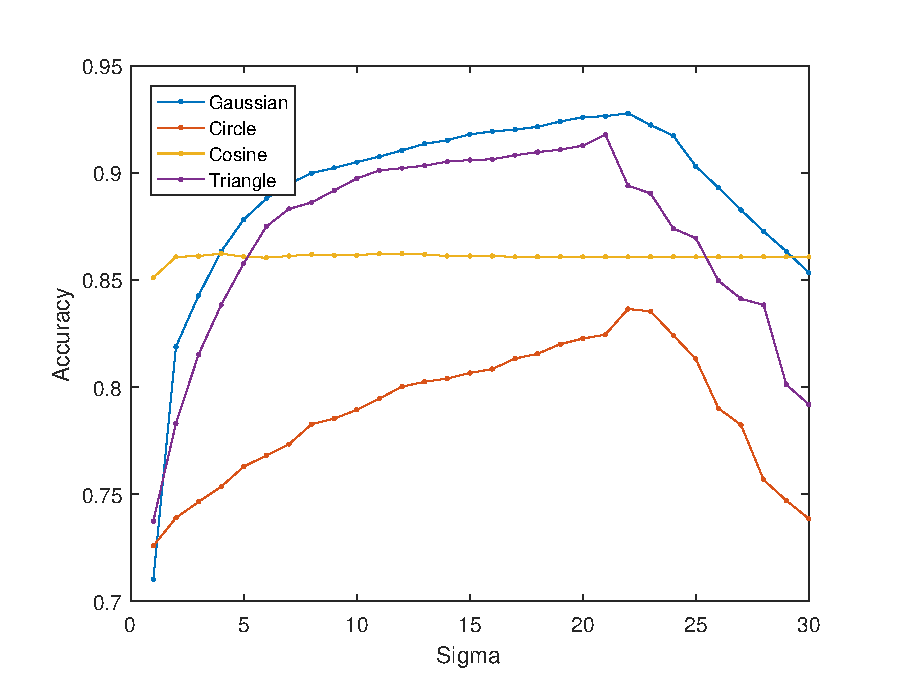
\includegraphics[width=0.5\textwidth,height=1.6in]{sigma.eps}
    \setlength{\abovecaptionskip}{-0.1cm}
    \caption{For different kernel functions, the relationship between sentiment analysis accuracy and $\sigma$}\label{fig:sigma}
\end{figure}

As shown in Fig~\ref{fig:sigma}, PESE-C is more stable and less affected by $\sigma$. Other three methods are more sensitive to the value of $\sigma$. For example, PESE-G achieves the highest accuracy of $92.77\%$ with $\sigma=21$.



\subsection{Evaluation of Public Opinion Model}
%shift detection 
First, we analyze the performance of shift detection. The ground truth of shift points for each incident is manually generated. Five volunteers observed the tweets at each time point and judged whether belongs to shift point. The final shift point gold standard is selected by taking a simple majority vote on each time points.

We compare our method with three state-of-the-art sentiment tracking methods. (1)POMS~\cite{Bollen2011sentimentchange}: measure sentiment polarity and calculate shift points with residuals. (2)FB-LDA~\cite{Tan2014topic}:  extract foreground topics from tweets in the variation period. (3)LDA \& KL-divergence~\cite{Giachanou2016sentichange}: extract topics in the time window and tank the topic based on their contribution.

%metric
We choose precision, recall and perplexity as evaluation metrics. The precision metric is shown as follows:

\begin{equation}
    Precision = \frac{time\;points\;with\;correct\;judgment}{time\;points\;with\;judgment}
\end{equation}

The purpose of precision can help us to judge how many time points are correctly judged.

\begin{equation}
    Recall = \frac{time\;points\;with\;judgment}{time\;points\;with\;judgment\;in\;the\;ground\;truth}
\end{equation}

Recall tells us how many time points we can judge whether belongs to shift point in the ground-truth.

\vspace{-0.6cm}
\begin{figure}
\centering
\subfigure[Precision]{\label{fig:precision}
    \centering
    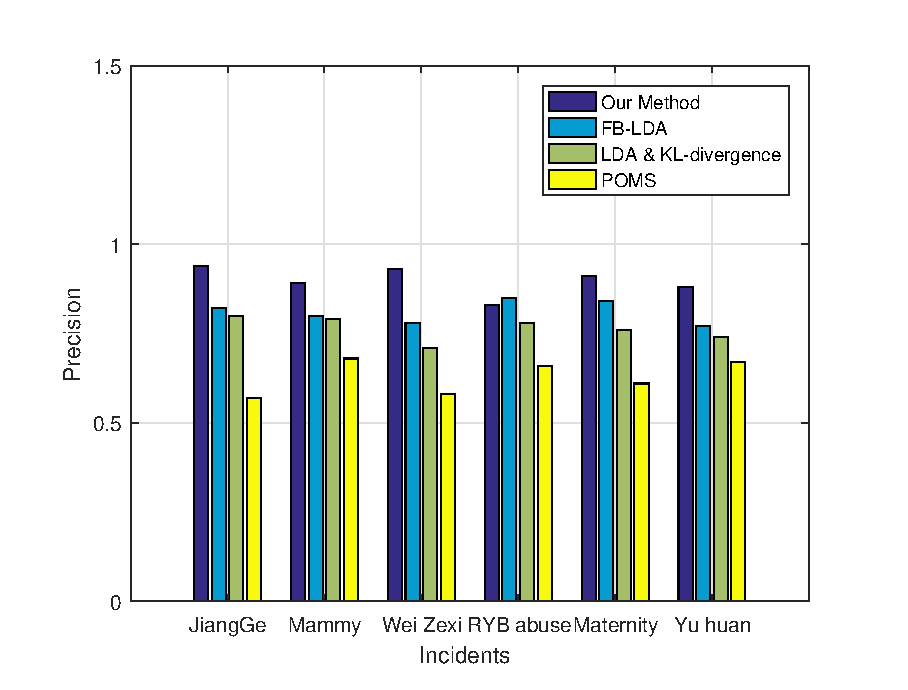
\includegraphics[width =.4\textwidth]{precision.eps}
}
\hspace{-4ex}
\subfigure[Recall]{\label{fig:recall}
    \centering
    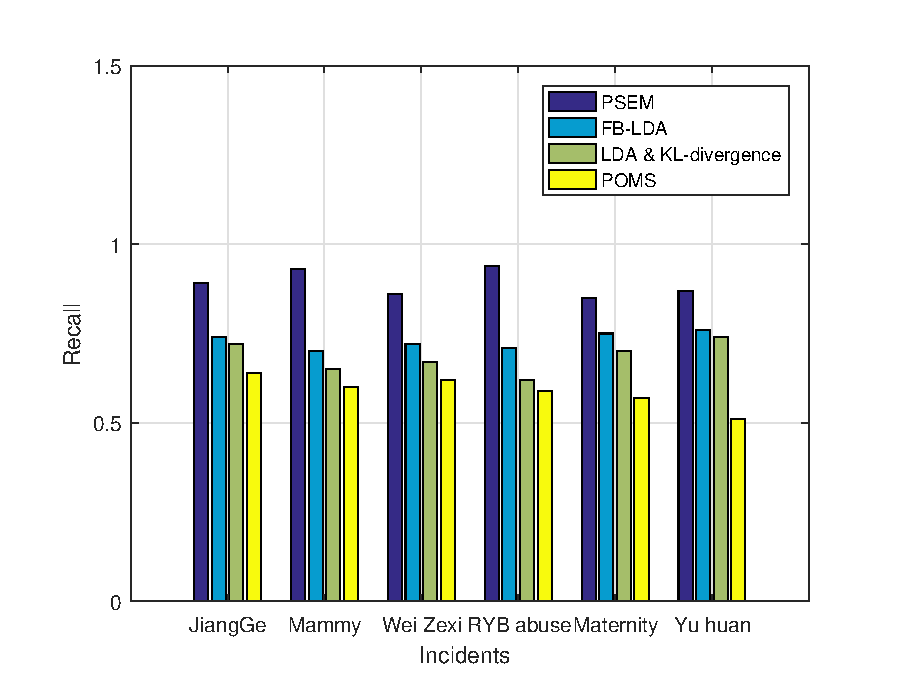
\includegraphics[width =.4\textwidth]{recall.eps}
}
\setlength{\abovecaptionskip}{-0.1cm}
\caption{Comparative performance of shift detection}\label{fig:shift}
\end{figure}

%result and analysis

As shown in Fig~\ref{fig:shift}, Our model has achieved the best results in detecting shift points. For the six events we selected, our model can achieve an average of 86\% precision and 90\% recall. In contrast, the average precision and recall of FB-LDA are 81\% and 73\%. For LDA \& KL-divergence are 76\% and 68\%. POMS performs the worst which the average precision and recall are 52\% and 59\%. These results show that our model can detect the public opinion shift in the incident more accurately.

%perplexity
Then, we analyze the performance of predictive. We choose perplexity as evaluation metric. 

\begin{equation}
    perplexity_{pw} = \exp\left\{-\frac{\sum_{d \in D}logp(w_d)}{\sum_{d \in D}N_d} \right\}
\end{equation}

Perplexity is a measurement of how well a probability distribution or probability model predicts a sample. A low perplexity indicates the probability distribution is good at predicting the sample. $p(w_d)$ is the probability of the $d$-th word. $N$ is the length of the sentence.

\vspace{-0.6cm}
\begin{figure}
    \centering
    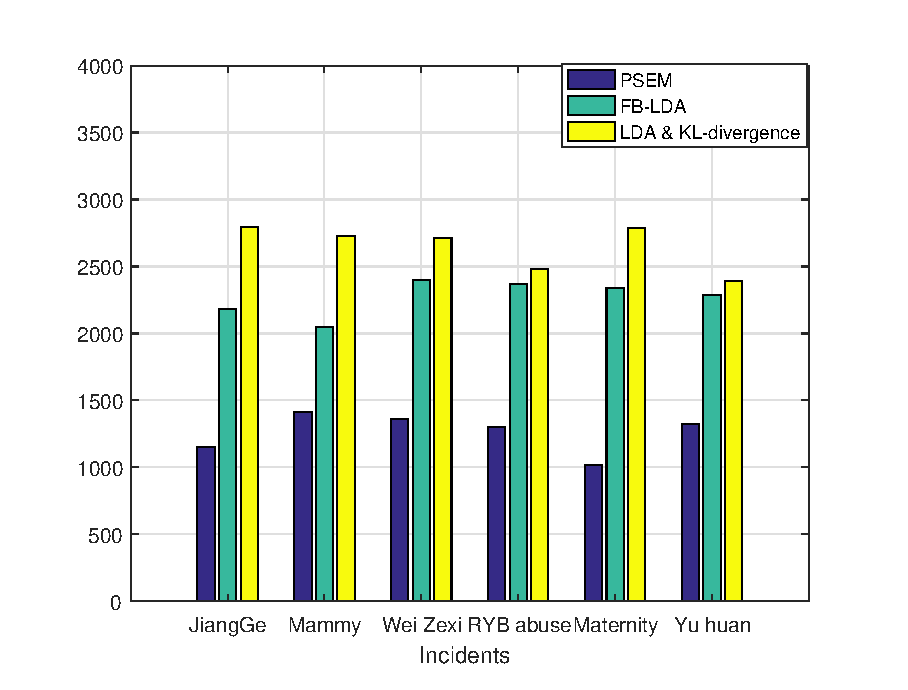
\includegraphics[width=0.5\textwidth,height=1.6in]{perplexity.eps}
    \setlength{\abovecaptionskip}{-0.1cm}
    \caption{Averaged per-word predictive perplexity comparison}\label{fig:perplexity}
\end{figure}

As shown in Fig~\ref{fig:perplexity},  Compared to the other two methods, our model has a smaller averaged per-word perplexity in all six incidents. This result indicates our model has better predictive performance.
%alpha

Finally, we offer visualization of the background sentiment evolution for the six incidents. 

\vspace{-0.6cm}
\begin{figure}
\centering
\subfigure[Maternity Fall]{\label{fig:time0}
    \centering
    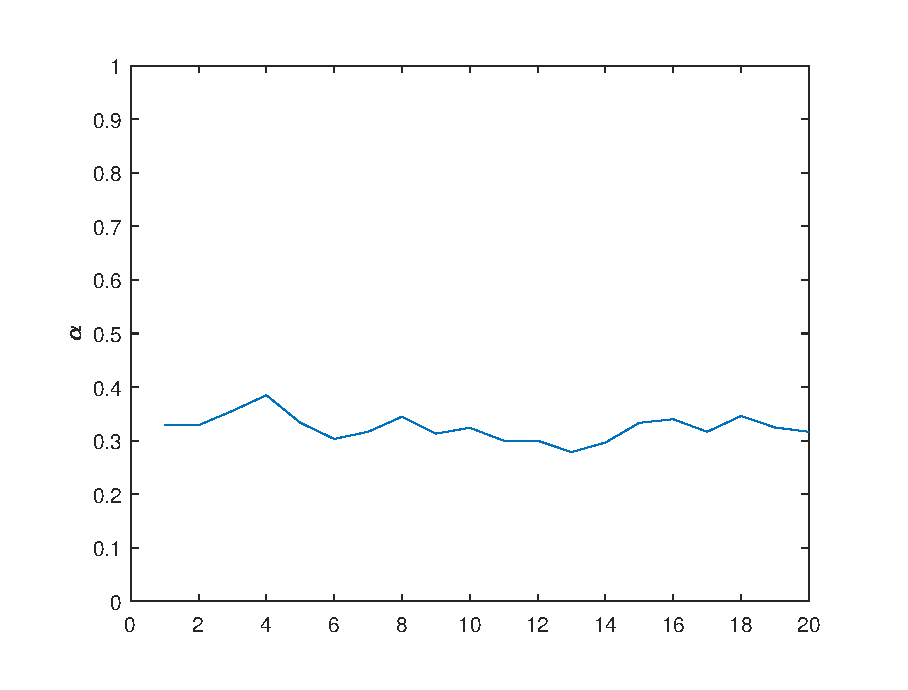
\includegraphics[width =.3\textwidth]{cfzla.eps}
}
\hspace{-0.15cm}
\subfigure[Kindergarten Abuse]{\label{fig:hhl}
    \centering
    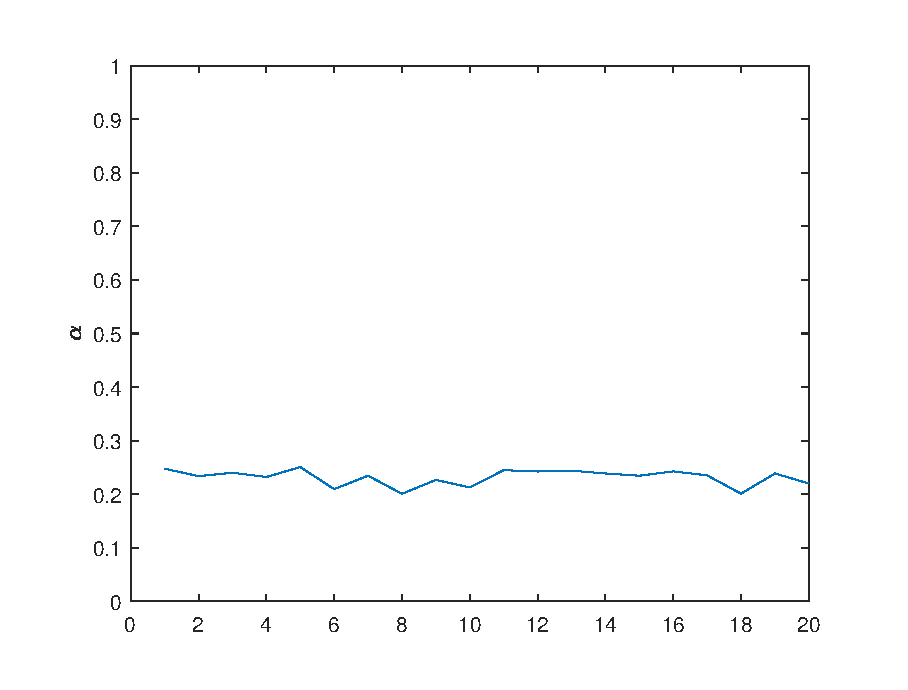
\includegraphics[width =.3\textwidth]{hhl.eps}
}
\hspace{-0.15cm}
\subfigure[Mammy Arson]{\label{fig:hzbml}
    \centering
    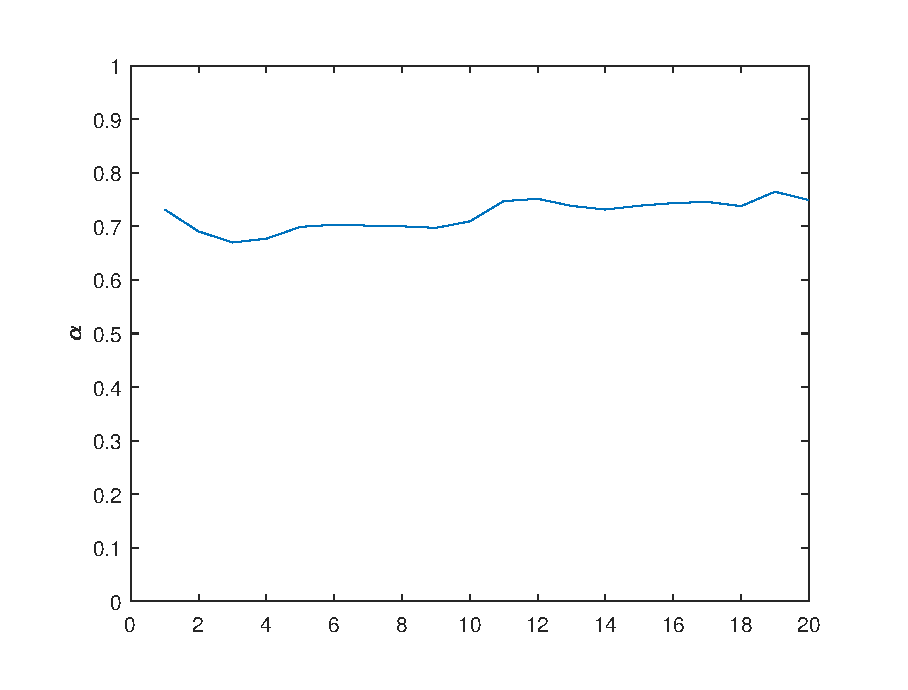
\includegraphics[width =.3\textwidth]{hzbm.eps}
}
\vspace{-0.3cm}
\subfigure[Jiang Ge Murder]{\label{fig:jg}
    \centering
    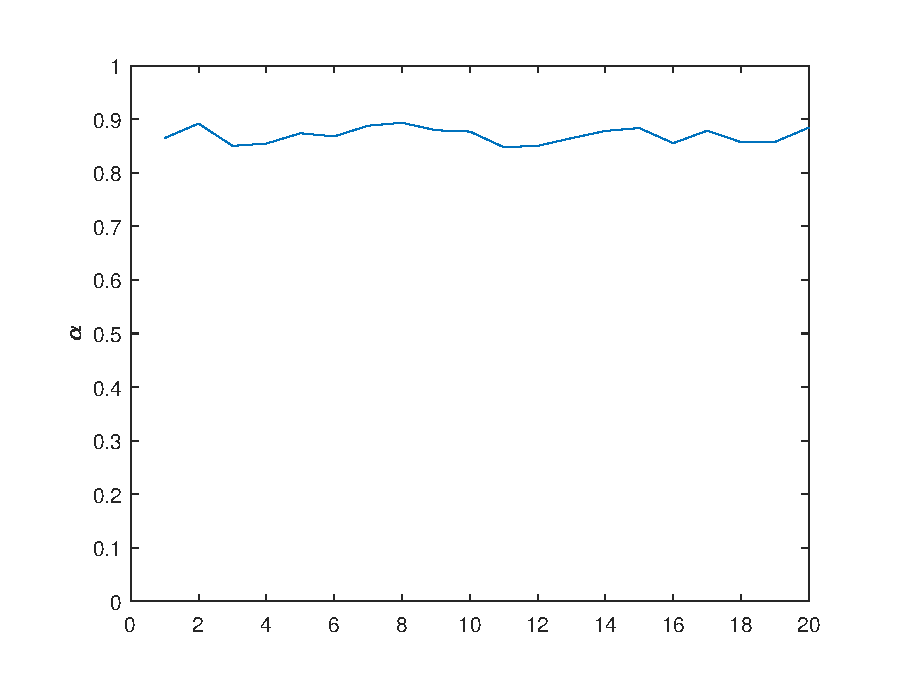
\includegraphics[width =.3\textwidth]{jg.eps}
}
\hspace{-0.15cm}
\subfigure[Yu Huan Murder]{\label{fig:sdrma}
    \centering
    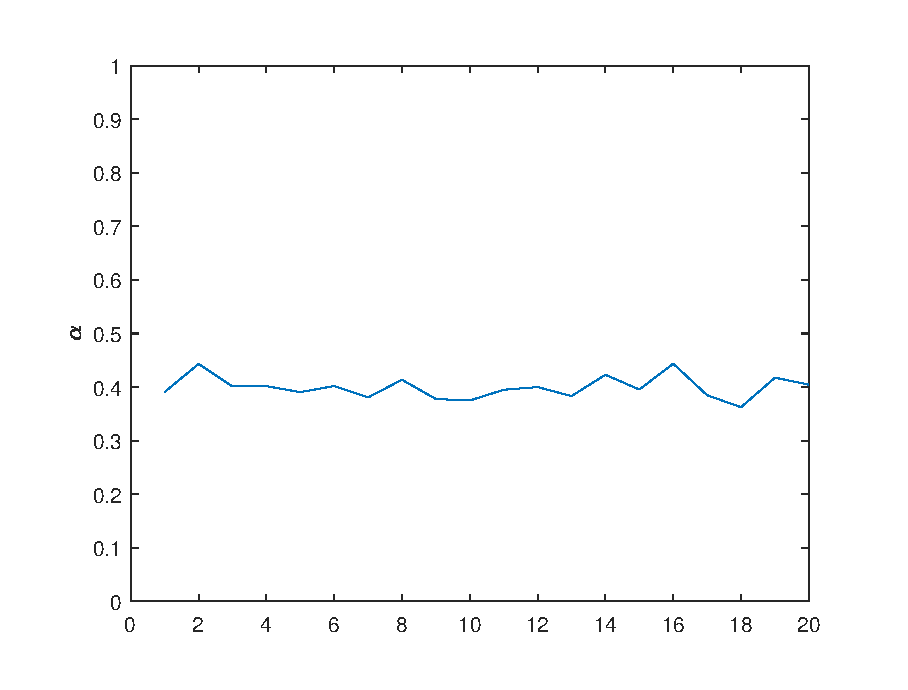
\includegraphics[width =.3\textwidth]{sdrma.eps}
}
\hspace{-0.15cm}
\subfigure[Death Of Wei Zexi]{\label{fig:wzx}
    \centering
    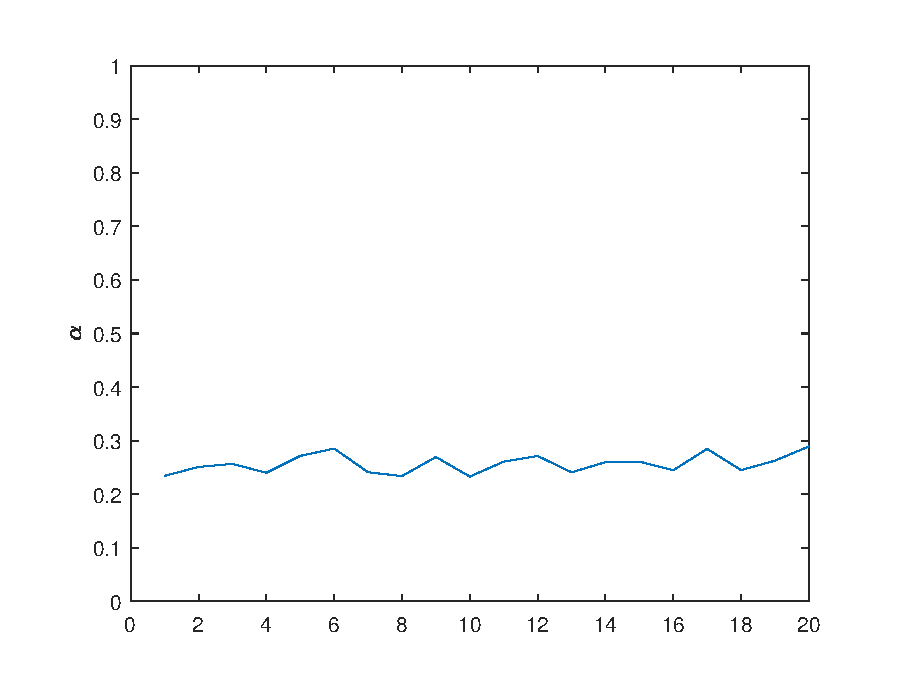
\includegraphics[width =.3\textwidth]{wzx.eps}
}
\caption{Changes in the $\alpha$ value of six incidents}\label{fig:alpha}
\end{figure}



As shown in Fig~\ref{fig:alpha}, the $\alpha$ which represents the distribution of background opinion in the incidents is smoothly and slowly changing in all six incidents as we considered before. The $\alpha$ of Death Of Wei Zexi, Kindergarten Abuse, Maternity Fall, and Yu Huan Murder is less than 0.5, indicating that negative sentiment is the back ground opinion to these incidents. The $\alpha$ of Jiang Ge Murder and Mammy Arson are greater than 0.5, indicating that positive sentiment is the back ground opinion to these incidents.











 

\section{Conclusion}\label{sec:conclusion}
In this paper, we study the problem of tracking the evolution of public opinion in social events. We analyze the differences between social events and entities in sentiment analysis, and propose a new opinion evolution model to track the changes in public opinion in social events. We consider the existence of background opinion distribution in the model, and use probability to indicate the likelihood of sudden changes in sentiments at each time point. To improve the performance of our model, we add entities in the process of sentiment analysis, use the distance function to calculate the influence of emotional words on entities, and experimentally prove that the distance function is more effective for long comments.

\begin{thebibliography}{8}
\bibitem{Cheung2014Battle}
Cheung A S Y. 
\newblock The Battle of Microblogging for Legal Justice in China. 
\newblock Ssrn Electronic Journal, 2014.

\bibitem{Giachanou2016sentichange}
Anastasia Giachanou, Ida Mele and Fabio Crestani.
\newblock  Explaining Sentiment Spikes in Twitter.
\newblock In CIKM ’16, PP. 2263-2268, 2016.

\bibitem{Giachanou2017sentichange}
Anastasia Giachanou, Ida Mele and Fabio Crestani.
\newblock  A Collection for Detecting Triggers of Sentiment Spikes.
\newblock In SIGIR ’17, PP. 1249-1252, 2017.

\bibitem{Tsytsarau2014Topics}
Mikalai Tsytsarau, Themis Palpanas and Malu Castellanos.
\newblock  Dynamics of news events and social media reaction.
\newblock In KDD ’14, PP. 901-910, 2014.

\bibitem{Thelwall2011topic}
Mike Thelwall, Kevan Buckley, and Georgios Paltoglou.
\newblock Sentiment in Twitter Events.
\newblock In Journal, pp. 406-418, 2011.

\bibitem{sentistrength2010}
Mike Thelwall,Kevan Buckley,Georgios Paltoglou,Di Cai,Arvid Kappas.
\newblock Sentiment strength detection in short informal text.
\newblock In Journa, pp. 2544–2558, 2010.

\bibitem{Thelwall2012lexicon}
Mike Thelwall, Kevan Buckley, and Georgios Paltoglou. 2012.
\newblock Sentiment strength detection for the social web.
\newblock J. Am. Soc. Inform. Sci. Technol. 63, 1 (2012), 163–173.

\bibitem{Ortega2013lexicon}
Reynier Ortega, Adrian Fonseca, and Andres Montoyo. 2013.
\newblock SSA-UO: Unsupervised twitter sentiment analysis.
\newblock In Proceedings of the 7th International Workshop on Semantic Evaluation.

\bibitem{Giachanou2016sentitime}
Anastasia Giachanou, Fabio Crestani. 2011.
\newblock Tracking Sentiment by Time Series Analysis.
\newblock In SIGIR ’16, pp. 1037-1040, 2016

\bibitem{An2014sentimentchange}
X. An, R. A. Ganguly, Y. Fang, B. S. Scyphers, M. A. Hunter, and G. J.
\newblock Tracking Climate Change Opinions from Twitter Data. 
\newblock In KDD’14, 2014.

\bibitem{Bollen2011sentimentchange}
J. Bollen, A. Pepe, and H. Mao.
\newblock Modeling Public Mood and Emotion : Twitter Sentiment and Socio-Economic Phenomena. 
\newblock In ICWSM’11, pages 450-453, 2011.

\bibitem{Tan2014topic}
Shulong Tan, Yang Li, Huan Sun, Ziyu Guan.
\newblock Interpreting the Public Sentiment Variations on Twitter. 
\newblock In Journal’14, 2014.

\bibitem{Montero2016sentimentchange}
C. S. Montero, H. Haddad, M. Mozgovoy, and C. B. Ali.
\newblock Detecting the likely causes behind the emotion spikes of influential twitter users. 
\newblock In CICLing’16, 2016.

\bibitem{Ahmed2017SentiCR}
Toufique Ahmed,Amiangshu Bosu,Anindya Iqbal,Shahram Rahimi.
\newblock SentiCR:A Customized Sentiment Analysis Tool for Code Review Interactions.
\newblock In ASE ’17.

\bibitem{Go2009Supervisedlearning}
Alec Go, Richa Bhayani, and Lei Huang. 2009.
\newblock Twitter Sentiment Classification Using Distant Supervision.
\newblock Technical Report. Standford.

\bibitem{Barbosa2010Supervisedlearning}
Luciano Barbosa and Junlan Feng.2010.
\newblock Robust sentiment detection on twitter from biased and noisy data.
\newblock In COLING ’10, pp. 36-44, 2010.

\bibitem{Papadopoulos2012SocialEvent}
Efthymios Kouloumpis, Theresa Wilson, and Johanna Moore. 2011.
\newblock Twitter sentiment analysis: The good the bad and the omg!
\newblock In ICWSM’11, pp. 538-541.

\bibitem{Pak2010Supervisedlearning}
Alexander Pak and Patrick Paroubek. 2010.
\newblock Twitter as a corpus for sentiment analysis and opinion mining.
\newblock In LREC ’10, pp. 1320-1326, 2010.

\bibitem{Davidov2010Supervisedlearning}
Dmitry Davidov, Oren Tsur, and Ari Rappoport.2010.
\newblock Enhanced sentiment learning using twitter hashtags and smileys.
\newblock In COLING ’10, pp. 241-249, 2010.

\bibitem{Agarwal2010Supervisedlearning}
Apoorv Agarwal, Boyi Xie, Ilia Vovsha, Owen Rambow, and Rebecca Passonneau. 2010.
\newblock Sentiment analysis of twitter data.
\newblock In LCM’11, pp. 30–38.

\bibitem{Hutto2014SSimproved}
C. J. Hutto and E. Gilbert. 2014.
\newblock Vader: A parsimonious rule-based model for sentiment analysis of social media text.
\newblock In AAAI’14.

\bibitem{Rakibul2017SentiStrength-SE}
Md Rakibul Islam and Minhaz F Zibran. 2017.
\newblock Leveraging automated sentiment analysis in software engineering. 
\newblock In Proceedings of IEEE Press, 203-214.

\bibitem{Feng2011lexicon}
Song Feng, Ritwik Bose, and Yejin Choi. 2011.
\newblock Learning general connotation of words using graph-based algorithms.
\newblock In EMNLP ’11, pp. 1092-1103, 2011.

\bibitem{Zhang2012corenodes}
Tiantian Zhang, Bin Wu.
\newblock A Method for Local Community Detection by Finding Core Nodes. \newblock In Proceedings of the 2012 IEEE/ACM 

\bibitem{Lv2009distancefunction}
Yuanhua Lv, ChengXiang Zhai.
\newblock Positional language models for information retrieval.
\newblock In SIRIG ’09, pp. 299-306, 2009.


\end{thebibliography}

\end{document}